% Options for packages loaded elsewhere
\PassOptionsToPackage{unicode}{hyperref}
\PassOptionsToPackage{hyphens}{url}
%
\documentclass[
]{article}
\usepackage{lmodern}
\usepackage{amssymb,amsmath}
\usepackage{ifxetex,ifluatex}
\ifnum 0\ifxetex 1\fi\ifluatex 1\fi=0 % if pdftex
  \usepackage[T1]{fontenc}
  \usepackage[utf8]{inputenc}
  \usepackage{textcomp} % provide euro and other symbols
\else % if luatex or xetex
  \usepackage{unicode-math}
  \defaultfontfeatures{Scale=MatchLowercase}
  \defaultfontfeatures[\rmfamily]{Ligatures=TeX,Scale=1}
\fi
% Use upquote if available, for straight quotes in verbatim environments
\IfFileExists{upquote.sty}{\usepackage{upquote}}{}
\IfFileExists{microtype.sty}{% use microtype if available
  \usepackage[]{microtype}
  \UseMicrotypeSet[protrusion]{basicmath} % disable protrusion for tt fonts
}{}
\makeatletter
\@ifundefined{KOMAClassName}{% if non-KOMA class
  \IfFileExists{parskip.sty}{%
    \usepackage{parskip}
  }{% else
    \setlength{\parindent}{0pt}
    \setlength{\parskip}{6pt plus 2pt minus 1pt}}
}{% if KOMA class
  \KOMAoptions{parskip=half}}
\makeatother
\usepackage{xcolor}
\IfFileExists{xurl.sty}{\usepackage{xurl}}{} % add URL line breaks if available
\IfFileExists{bookmark.sty}{\usepackage{bookmark}}{\usepackage{hyperref}}
\hypersetup{
  pdftitle={Asynchronous Transfer Mode (ATM) Networks},
  hidelinks,
  pdfcreator={LaTeX via pandoc}}
\urlstyle{same} % disable monospaced font for URLs
\usepackage{graphicx}
\makeatletter
\def\maxwidth{\ifdim\Gin@nat@width>\linewidth\linewidth\else\Gin@nat@width\fi}
\def\maxheight{\ifdim\Gin@nat@height>\textheight\textheight\else\Gin@nat@height\fi}
\makeatother
% Scale images if necessary, so that they will not overflow the page
% margins by default, and it is still possible to overwrite the defaults
% using explicit options in \includegraphics[width, height, ...]{}
\setkeys{Gin}{width=\maxwidth,height=\maxheight,keepaspectratio}
% Set default figure placement to htbp
\makeatletter
\def\fps@figure{htbp}
\makeatother
\setlength{\emergencystretch}{3em} % prevent overfull lines
\providecommand{\tightlist}{%
  \setlength{\itemsep}{0pt}\setlength{\parskip}{0pt}}
\setcounter{secnumdepth}{-\maxdimen} % remove section numbering

\title{Asynchronous Transfer Mode (ATM) Networks}
\author{}
\date{}

\begin{document}
\maketitle

\hypertarget{what-is-atm}{%
\subsection{What is ATM?}\label{what-is-atm}}

Asynchronous Transfer Mode (ATM) is a high-speed networking technology
that uses fixed-size cells of 53 bytes to transmit data. Each ATM cell
consists of a 5-byte header and a 48-byte payload.

ATM operates at the \textbf{\emph{data link layer}} (Layer 2) of the OSI
model, and it is \textbf{\emph{connection-oriented}}, meaning it
\emph{establishes a virtual connection between endpoints before data
transmission begins}. ATM is known for its ability to provide
\textbf{Quality of Service (QoS)} guarantees, making it suitable for
real-time applications like voice and video conferencing.

\hypertarget{charactersitics}{%
\subsection{Charactersitics:}\label{charactersitics}}

\begin{itemize}
\tightlist
\item
  Sender establishes a \emph{virtual circuit} connection to receiver(s)
\item
  Route is determined and \emph{routing information stored in switches}
\item
  Data is divided into small, fixed-size units called \textbf{cells}
\end{itemize}

\hypertarget{advantages-of-atm}{%
\subsection{Advantages of ATM:}\label{advantages-of-atm}}

\begin{itemize}
\tightlist
\item
  Single network \emph{can transport multiple types of data} (voice,
  video, data, etc.)
\item
  Integration of services leads to cost savings
\item
  Enables new applications like \emph{video-on-demand} and
  \emph{teleconferencing}
\item
  Efficient for \emph{broadcasting to multiple destinations
  simultaneously}.
\end{itemize}

\hypertarget{benefits-of-fixed-size-cells}{%
\subsection{Benefits of fixed-size
cells:}\label{benefits-of-fixed-size-cells}}

\begin{itemize}
\tightlist
\item
  Allow \emph{rapid switching}
\item
  Eliminate delays caused by large packets blocking lines
\item
  New cells can be sent immediately after each transmission
\end{itemize}

\hypertarget{comparison-to-traditional-methods}{%
\subsection{Comparison to traditional
methods:}\label{comparison-to-traditional-methods}}

\begin{itemize}
\tightlist
\item
  More flexible than conventional circuit switching
\item
  Better suited for broadcast media than telephone systems
\item
  Can handle \textbf{point-to-point} and \textbf{multicasting}
  efficiently
\end{itemize}

\hypertarget{atm-layers}{%
\subsection{ATM Layers}\label{atm-layers}}

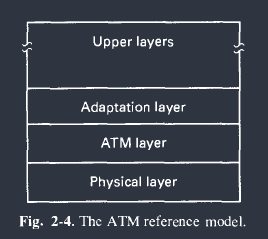
\includegraphics{/home/abishai/Documents/NotesObs/DOS/Pasted image 20240819221223.png}

\hypertarget{physical-layer}{%
\subsubsection{1. Physical Layer}\label{physical-layer}}

\begin{itemize}
\tightlist
\item
  It is responsible for the \emph{transmission and reception of raw
  bitstreams over a physical medium}.
\item
  Empty cells are transmitted when no data is available
\item
  ATM is \emph{synchronous at the physical layer}, but
  \emph{asynchronous within virtual circuits}
\item
  \textbf{SONET (Synchronous Optical NETwork)}:

  \begin{itemize}
  \tightlist
  \item
    Used in the physical layer for ATM
  \item
    \emph{ATM cells are placed in the payload portion of SONET frames}
  \item
    Compatible with AT\&T and other carriers' internal transmission
    systems
  \item
    In Europe, a similar system called \emph{SDH} is used
  \end{itemize}
\item
  ATM and SONET unlikely for audio telephones (ISDN used instead)
\item
  ATM and SONET considered ideal for videophones
\end{itemize}

\hypertarget{atm-layer}{%
\subsubsection{2. ATM Layer}\label{atm-layer}}

\begin{itemize}
\tightlist
\item
  The ATM layer is responsible for the cell-based transmission. It deals
  with the transmission, and switching of small, fixed-sized packets
  called \textbf{ATM cells}. Each cell is 53 bytes long, consisting of a
  5-byte header and a 48-byte payload.
\item
  This layer handles functions like \emph{cell multiplexing}, \emph{cell
  switching}, and the maintenance of \emph{Quality of Service (QoS)}.
\end{itemize}

\hypertarget{header-layout}{%
\paragraph{Header Layout:}\label{header-layout}}

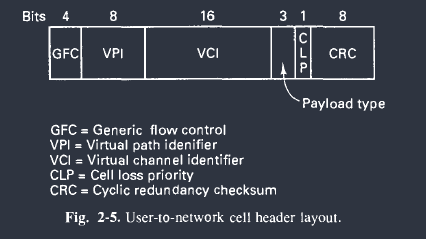
\includegraphics{/home/abishai/Documents/NotesObs/DOS/Pasted image 20240819222956.png}

\begin{itemize}
\tightlist
\item
  \textbf{Fields}:

  \begin{itemize}
  \tightlist
  \item
    \textbf{\emph{GFC}}: May be used for \emph{flow control} in the
    future
  \item
    \textbf{\emph{VPI}} and \textbf{\emph{VCI}}: Identify \emph{path and
    virtual circuit for routing}
  \item
    \textbf{\emph{Payload type}}: \emph{Distinguishes data cells from
    control cells}
  \item
    \textbf{\emph{CLP}}: Marks cell \emph{importance for congestion}
    (lower priority cells dropped first)
  \item
    \textbf{\emph{CRC}}: 1-byte checksum over the header
  \end{itemize}
\item
  GFC field in computer-to-switch replaced by four more VPI bits in
  switch-to-switch
\item
  Both types have 48-byte payloads following the header
\item
  Fields modified at each hop
\item
  VPI groups virtual circuits for the same destination
\end{itemize}

\hypertarget{adaptation-layer-aal---atm-adaptive-layer}{%
\subsubsection{3. Adaptation Layer (AAL - ATM Adaptive
Layer)}\label{adaptation-layer-aal---atm-adaptive-layer}}

\begin{itemize}
\tightlist
\item
  \emph{Handles segmentation and reassembly of data, error detection,
  and the handling of timing issues.}
\item
  Need for Adaptation Layer:

  \begin{itemize}
  \tightlist
  \item
    At 155 Mbps, a cell arrives every 3 μsec
  \item
    Most CPUs can't handle 300,000 interrupts/sec
  \item
    Adaptation layer \emph{breaks packets into cells and reassembles
    them}, generating \emph{one interrupt per packet instead of per
    cell}
  \end{itemize}
\item
  Adaptation layer runs on the \textbf{host adaptor board}
\item
  \textbf{Traffic Classes} (\emph{bit rate} \& \emph{data traffic}):

  \begin{enumerate}
  \tightlist
  \item
    Constant bit rate (for audio and video)
  \item
    Variable bit rate with bounded delay
  \item
    Connection-oriented data traffic
  \item
    Connectionless data traffic
  \end{enumerate}
\item
  Evolution of Classes:

  \begin{itemize}
  \tightlist
  \item
    Classes 3 and 4 were merged into a new class 3/4
  \item
    Computer industry proposed AAL 5 for computer-to-computer traffic
  \end{itemize}
\end{itemize}

\hypertarget{seal-simple-and-efficient-adaptation-layer-aal-5}{%
\paragraph{SEAL (Simple and Efficient Adaptation Layer) {[}AAL
5{]}:}\label{seal-simple-and-efficient-adaptation-layer-aal-5}}

\begin{itemize}
\tightlist
\item
  Nickname for AAL 5
\item
  Uses only one bit in the ATM header (Payload type field)
\item
  Bit is normally 0, set to 1 in the last cell of a packet
\item
  \textbf{Trailer (final 8 bytes)}: The trailer helps \emph{mark the end
  of a packet}. The last cell of a packet has its \emph{Payload type bit
  set to 1, indicating that it contains the trailer}. This allows the
  receiving end to know when a complete packet has been received.
\item
  \textbf{SEAL Packet Structure}:

  \begin{itemize}
  \tightlist
  \item
    Padding (zeros) may be added between packet end and trailer start
  \item
    Destination assembles incoming cells until it finds the
    end-of-packet bit
  \item
    Trailer is then extracted and processed
  \end{itemize}
\item
  \textbf{Trailer Structure}:

  \begin{itemize}
  \tightlist
  \item
    Four fields in total

    \begin{itemize}
    \tightlist
    \item
      First two fields (1 byte each) are unused
    \item
      2-byte field for \emph{packet length}
    \item
      4-byte \emph{checksum} over the packet, padding, and trailer
    \end{itemize}
  \end{itemize}
\end{itemize}

\hypertarget{upper-layer}{%
\subsubsection{4. Upper Layer}\label{upper-layer}}

\begin{itemize}
\tightlist
\item
  These are the layers above the adaptation layer, typically consisting
  of the network, transport, and application layers (e.g., IP, TCP,
  applications). These layers are not specific to ATM and are more
  related to the general OSI model or TCP/IP model. The adaptation layer
  ensures that these upper-layer protocols can effectively communicate
  over the ATM network.
\end{itemize}

\hypertarget{atm-switching-techniques}{%
\section{ATM Switching Techniques}\label{atm-switching-techniques}}

\begin{itemize}
\tightlist
\item
  ATM networks use \emph{copper} or \emph{optical} cables and switches.
\item
  A network can have multiple switches, each switch with four ports for
  input and output.\\
  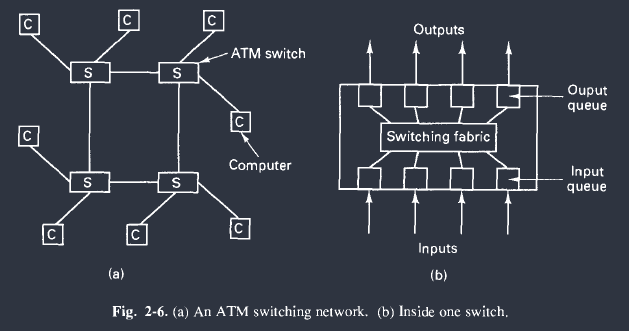
\includegraphics{/home/abishai/Documents/NotesObs/DOS/Pasted image 20240819233853.png}
\item
  Switches have input and output lines connected by a \emph{parallel
  switching fabric}.
\item
  Parallel switching is necessary due to the \emph{speed required} (3
  μsec at OC-3) and \emph{multiple simultaneous inputs}.
\item
  \textbf{Cell Routing}:

  \begin{itemize}
  \tightlist
  \item
    When a cell arrives, its VPI and VCI fields are examined to
    determine the correct output port.
  \item
    Cells must be delivered in order.
  \end{itemize}
\item
  \textbf{Head-of-line Blocking}:

  \begin{itemize}
  \tightlist
  \item
    This problem occurs when two \emph{cells arrive simultaneously on
    different input lines} but need the \emph{same output port}.
  \item
    Simply discarding one cell is inefficient.
  \item
    Solution:

    \begin{itemize}
    \tightlist
    \item
      A common solution is to \emph{randomly select one cell to forward
      and hold the other for the next round}.
    \item
      Some designs \emph{copy cells into output port queues instead of
      keeping them in input buffers}.
    \item
      Switches may use a \emph{pool of buffers for both input and
      output}.
    \item
      Input-side buffering with \emph{selective forwarding} is another
      option.
    \end{itemize}
  \end{itemize}
\item
  Other Switch Designs:

  \begin{itemize}
  \tightlist
  \item
    \textbf{Time division switches} using shared memory
  \item
    \textbf{Space division switches} with multiple paths between inputs
    and outputs
  \item
    Designs using \textbf{buses} or \textbf{rings}
  \end{itemize}
\end{itemize}

\hypertarget{implications-of-atm-on-distributed-systems}{%
\subsubsection{Implications of ATM on distributed
systems}\label{implications-of-atm-on-distributed-systems}}

\begin{enumerate}
\item
  \textbf{Impact of Bandwidth}: The availability of high bandwidth
  (e.g., 155 Mbps, 622 Mbps, and potentially 2.5 Gbps) creates
  significant implications for distributed systems, mainly due to the
  sudden availability of large bandwidths. This has pronounced effects
  on wide-area distributed systems, where \emph{latency becomes a
  critical issue}.
\item
  \textbf{Latency Concerns}: As network speeds increase, the
  time-to-reply decreases, but for very high-speed networks, it
  approaches zero, \emph{which means most of the time is spent waiting
  for acknowledgments}. For smaller messages, this issue becomes even
  more pronounced, leading to inefficiencies.

  \begin{itemize}
  \tightlist
  \item
    Even though high-speed networks can transmit large amounts of data
    quickly, delay is introduced by waiting for acknowledgments.
  \end{itemize}
\item
  \textbf{Flow Control Challenges}: Managing large files, such as a 10
  GB video, over ATM networks can be problematic. \emph{If buffer space
  is insufficient, data loss may occur, requiring retransmissions and
  potentially leading to inefficient use of bandwidth.} Traditional flow
  control methods, like sliding windows, may not be effective, leading
  to the need for new approaches.
\item
  \textbf{Transcontinental Delay}: The inherent delay in
  transcontinental communications (e.g., from New York to California)
  can significantly affect performance, especially when multiple
  sequential requests are made. This delay can lead to noticeable lag,
  which may prompt a rethink of distributed system architectures.
\item
  \textbf{Congestion and Cell Dropping}: ATM networks allow switches to
  drop cells when congested, which can cause significant problems,
  especially for services requiring uniform rates, like audio streaming.
\end{enumerate}

\end{document}
